\documentclass{article}
\usepackage[utf8]{inputenc}

\title{detectorhandins}
\author{Daniel S. Nielsen, Rosanna Ignazzi, \\Étienne Bourbeau, Fabian A.J. Thiele}
\date{October 2018}
\usepackage{siunitx} % SI units
\usepackage{amsmath} % equations
\usepackage{tabularx}
\usepackage{tikz}
\usepackage{hyperref}
\usepackage{ifthen}
\usepackage[T1]{fontenc} % proper underscores etc.
\usepackage{subcaption} % replace subfloat with subfigure env.
\usepackage{float}
\usepackage{todonotes}
\usepackage{placeins}
\setlength{\parskip}{.8em} % add some space btwn paragraphs


\sisetup{per-mode=fraction}

\begin{document}
	% === Front matter ====================================================

	%\frontmatter
	\maketitle
	
	\tableofcontents
	
	%\listoffigures
	
	%\listoftables
	
	%\lstlistoflistings
	
	\cleardoublepage
	\begin{abstract}
  This is a placeholder for the actual abstract.
  \todo[inline]{Insert correct abstract here.}
\end{abstract}
	
	\clearpage
	\section*{Introduction}  \label{sec:Introduction}
\addcontentsline{toc}{section}{\protect\numberline{}Introduction}

	
	
	
	
	% === Main matter =====================================================

        % Report structure reflects the structure laid out in todo.txt
	
	% --- Chapter 1: Background -----------------------------------------------
	
	\cleardoublepage

        \clearpage
	\section{Gas Detector construction}
\label{sec:construction}

\subsection{Cider can}
\subsubsection{Material preparation}
We have been handed a start-up kit consisting of one empty \SI{500}{\milli\liter}
cider can, two Plexiglas endcaps, two Teflon pipes, one nylon screw and nut,
brass pipes and a high voltage (HV) connector with a small exterior connector for
grounding the outside of the can.

\begin{table}[htb!]%
\begin{maybeleft}%
  \begin{tabularx}{\linewidth}{p{3.6cm}p{0.7cm}p{3cm}}
    \textbf{Element}       &               & \textbf{Mean} \\ \hline
    Can diameter           & $D_{outer}$   & $65.82 \pm 0.22$~mm     \\
    Can wall thickness     & $\tau$        & $\SI{105}{\micro\meter}$   \\
    Plastic tube diameter  & $d_{t}$       & $5.97 \pm 0.05$~mm       \\
    Brass tube diameter    & $d_{brass}$   & $1.0$~mm       \\
    Nylon screw diameter   & $d_{screw}$   & $7.78 \pm 0.04$~mm       \\
    HV connector diameter  & $d_{HV}$      & $9.37$~mm      \\
    Anode wire diameter    & $d_{wire}$    & $\SI{50}{\micro\meter}$    \\
    \hline
  \end{tabularx}
  \caption{Measurements of the cider can experiment setup components. Measurements without uncertainties were only measured once and are dominated by the systematic uncertainties of the measurement tools.}
  \label{Tab:cidercan_sizes}
\end{maybeleft}%
\end{table}

The process started with the preparation of the cider can which included cutting
away the top part of the can, removing the inner coating with a drill equipped with a
metal brush on top, drilling two holes in the bottom: one in the middle of the
endcap for the nylon screw and one slightly offset from the center for the
gas exchange system (of $d = \SI{8.0}{\milli\meter}$ and $d =
\SI{6.0}{\milli\meter}$). The second step consisted in drilling the necessary
holes in the Plexiglas endcaps (which already have a groove for the can
extremities to be fitted in): one hole for the gas Teflon pipe in the back
endcap and one for the front endcap, as well as a hole for the HV connector in the
front endcap (the diameters are $d = \SI{6.0}{\milli\meter}$ and $d =
\SI{9.5}{\milli\meter}$ respectively). Finally a small hole of $d =
\SI{1.0}{\milli\meter}$ was drilled in the Teflon screw, in order to insert the
brass pipe in there at a later point. The brass tubes were cut and flattened
with sand paper, to remove the part that was squeezed due to the cutting tool.

\begin{figure}[htb!]
  \centering
  \includegraphics[width=0.5\textwidth]{./graphics/brass_file.jpg}
  \caption{Filing of the brass tube}
  \label{fig:brass_file}
\end{figure}


Once all the ingredients were ready, all the holes in the can and the edges of
the brass tube were filed and checked under a microscope (see \ref{fig:brass_file}), in order to avoid
sharp edges. All the components were placed in an isopropanol (IPA) bath in a
sonicator, so all the skin oils and dirt were cleaned off, and the parts were
dried with $\mathrm{N}_2$ gas. At this point, the only element missing was the
anode wire, which was taken from a regular low voltage cable and carefully wiped
with a cloth dipped in IPA.


\subsubsection{Assembly}

The assembly of the detector started with the fastening of the nylon screw and
bolt to the aluminium can, using the hole in the middle of the bottom of the
can. The longer of the two brass tubes was inserted in the nylon screw, and one
end of the anode wire was passed in the brass tube from the outside and pulled
until the other end of the can. On the other extremity of the anode wire, a
small nut was attached with a simple knot, in order to help keeping the anode
wire straight later on in the process. The free end of the wire was inserted in
the shorter brass tube and both were soldered to the HV connector, which
had been previously fastened to the front Plexiglas endcap (a small contact
has been placed between the HV connector and the outer glass, to later
use it for grounding the cathode). The front endcap was glued with epoxy to the
cider can and was left to dry for some time. The next step consisted in
straightening out the anode wire inside the can by pulling it slowly out of the
can from the bottom. The wire has to be quite straight in order to avoid dips,
where the charge could concentrate and obscure the measurement. To reach an
optimal condition, a weight was carefully lowered to slowly apply tension.
When a satisfactory straightness was achieved, the wire was soldered to the
brass pipe and the rest cut off. The back endcap was glued to the cider can and
left to dry for some time.

The gas Teflon tubes were glued to the front and back endcap and a small
quantity of glue was applied around the HV connector, to ensure optimal
insulation.

Before moving on to the next step, a leakage test was performed, to check for
possible holes in the glue. The gas supply (in our case $\mathrm{P}_{10}$) was
attached to one of the Teflon gas tubes and to a flowmeter, which measured a gas
flow of approximately \SI{25}{\milli\liter\per\minute} out of the tube. When
moving the flowmeter to the other end of the can detector, the gas flow measured
was between \SIrange{2}{4}{\milli\liter\per\min}, which meant that an extra layer
of glue had to be applied to the outside and the endcaps and to the tube
connections, to cover potential leaks. After this adjustment, the gas
flow was measured again and the gas flow injected in the detector was
\SI{18.3}{\milli\liter\per\minute}, while the outgoing gas flow was of
\SI{17.6}{\milli\liter\per\minute}. This was determined to be sufficient for the
purpose of the experiment.

The last step consisted in removing some of the coating from the outside of the cider can with sand paper, and connecting the grounding pin previously attached
to the HV connector to the bare aluminium of the can with copper tape. This tape would later be grounded to the cathode to create the electric field inside the can. The
connection was checked with a multimeter, where it was asserted, that there is no connection between the cathode can and the anode wire.

\subsection{Copper Tube}
\subsubsection{Assembly}
A more sophisticated detector made out of copper was built after the more rudimentary one. In this iteration of the gas counter, the proportional chamber experiment was made out of a machined copper tube. The end caps were made out of two Teflon plugs, brass tubes were again used as electric field protector, and a finer, copper beryllium wire was selected as the anode material. The material also included smaller Teflon pipes for the gas inlets, and the same HV connector and a the same grounding pin as the cider can assembly. Figure \ref{fig:copper_parts} shows all parts of the assembly.

In order to ensure that the X-ray emission from the source would be able to penetrate the thicker walls of the copper tube, a hole of $5$ mm was drilled in the copper tube, approximately in the middle of the pipe. The Teflon plugs were filed down in order to match the inner radius of the copper pipe and the pre-existing holes for the gas supply tubes. The HV connector and brass tube were adjusted to the appropriate sizes of the different components. Similarly to the previous detector, the brass pipe was sanded and filed at the edges to remove any sharp debris that would cause sparking.

All the parts were cleaned in an IPA bath and dried with N$_2$. The wire was soldered to the brass tube and to the HV connector and inserted carefully in the copper tube. This part of the procedure was much more delicate than in the previous assembly, given the tendency of the much thinner wire to curl on itself and break easily. The copper tube was glued with epoxy to the front Teflon plug. The wire was then passed into the second brass tube and in the back Teflon plug  The back plug was glued and the wire soldered to the brass tube.

\begin{figure}[htb!]
  \centering
  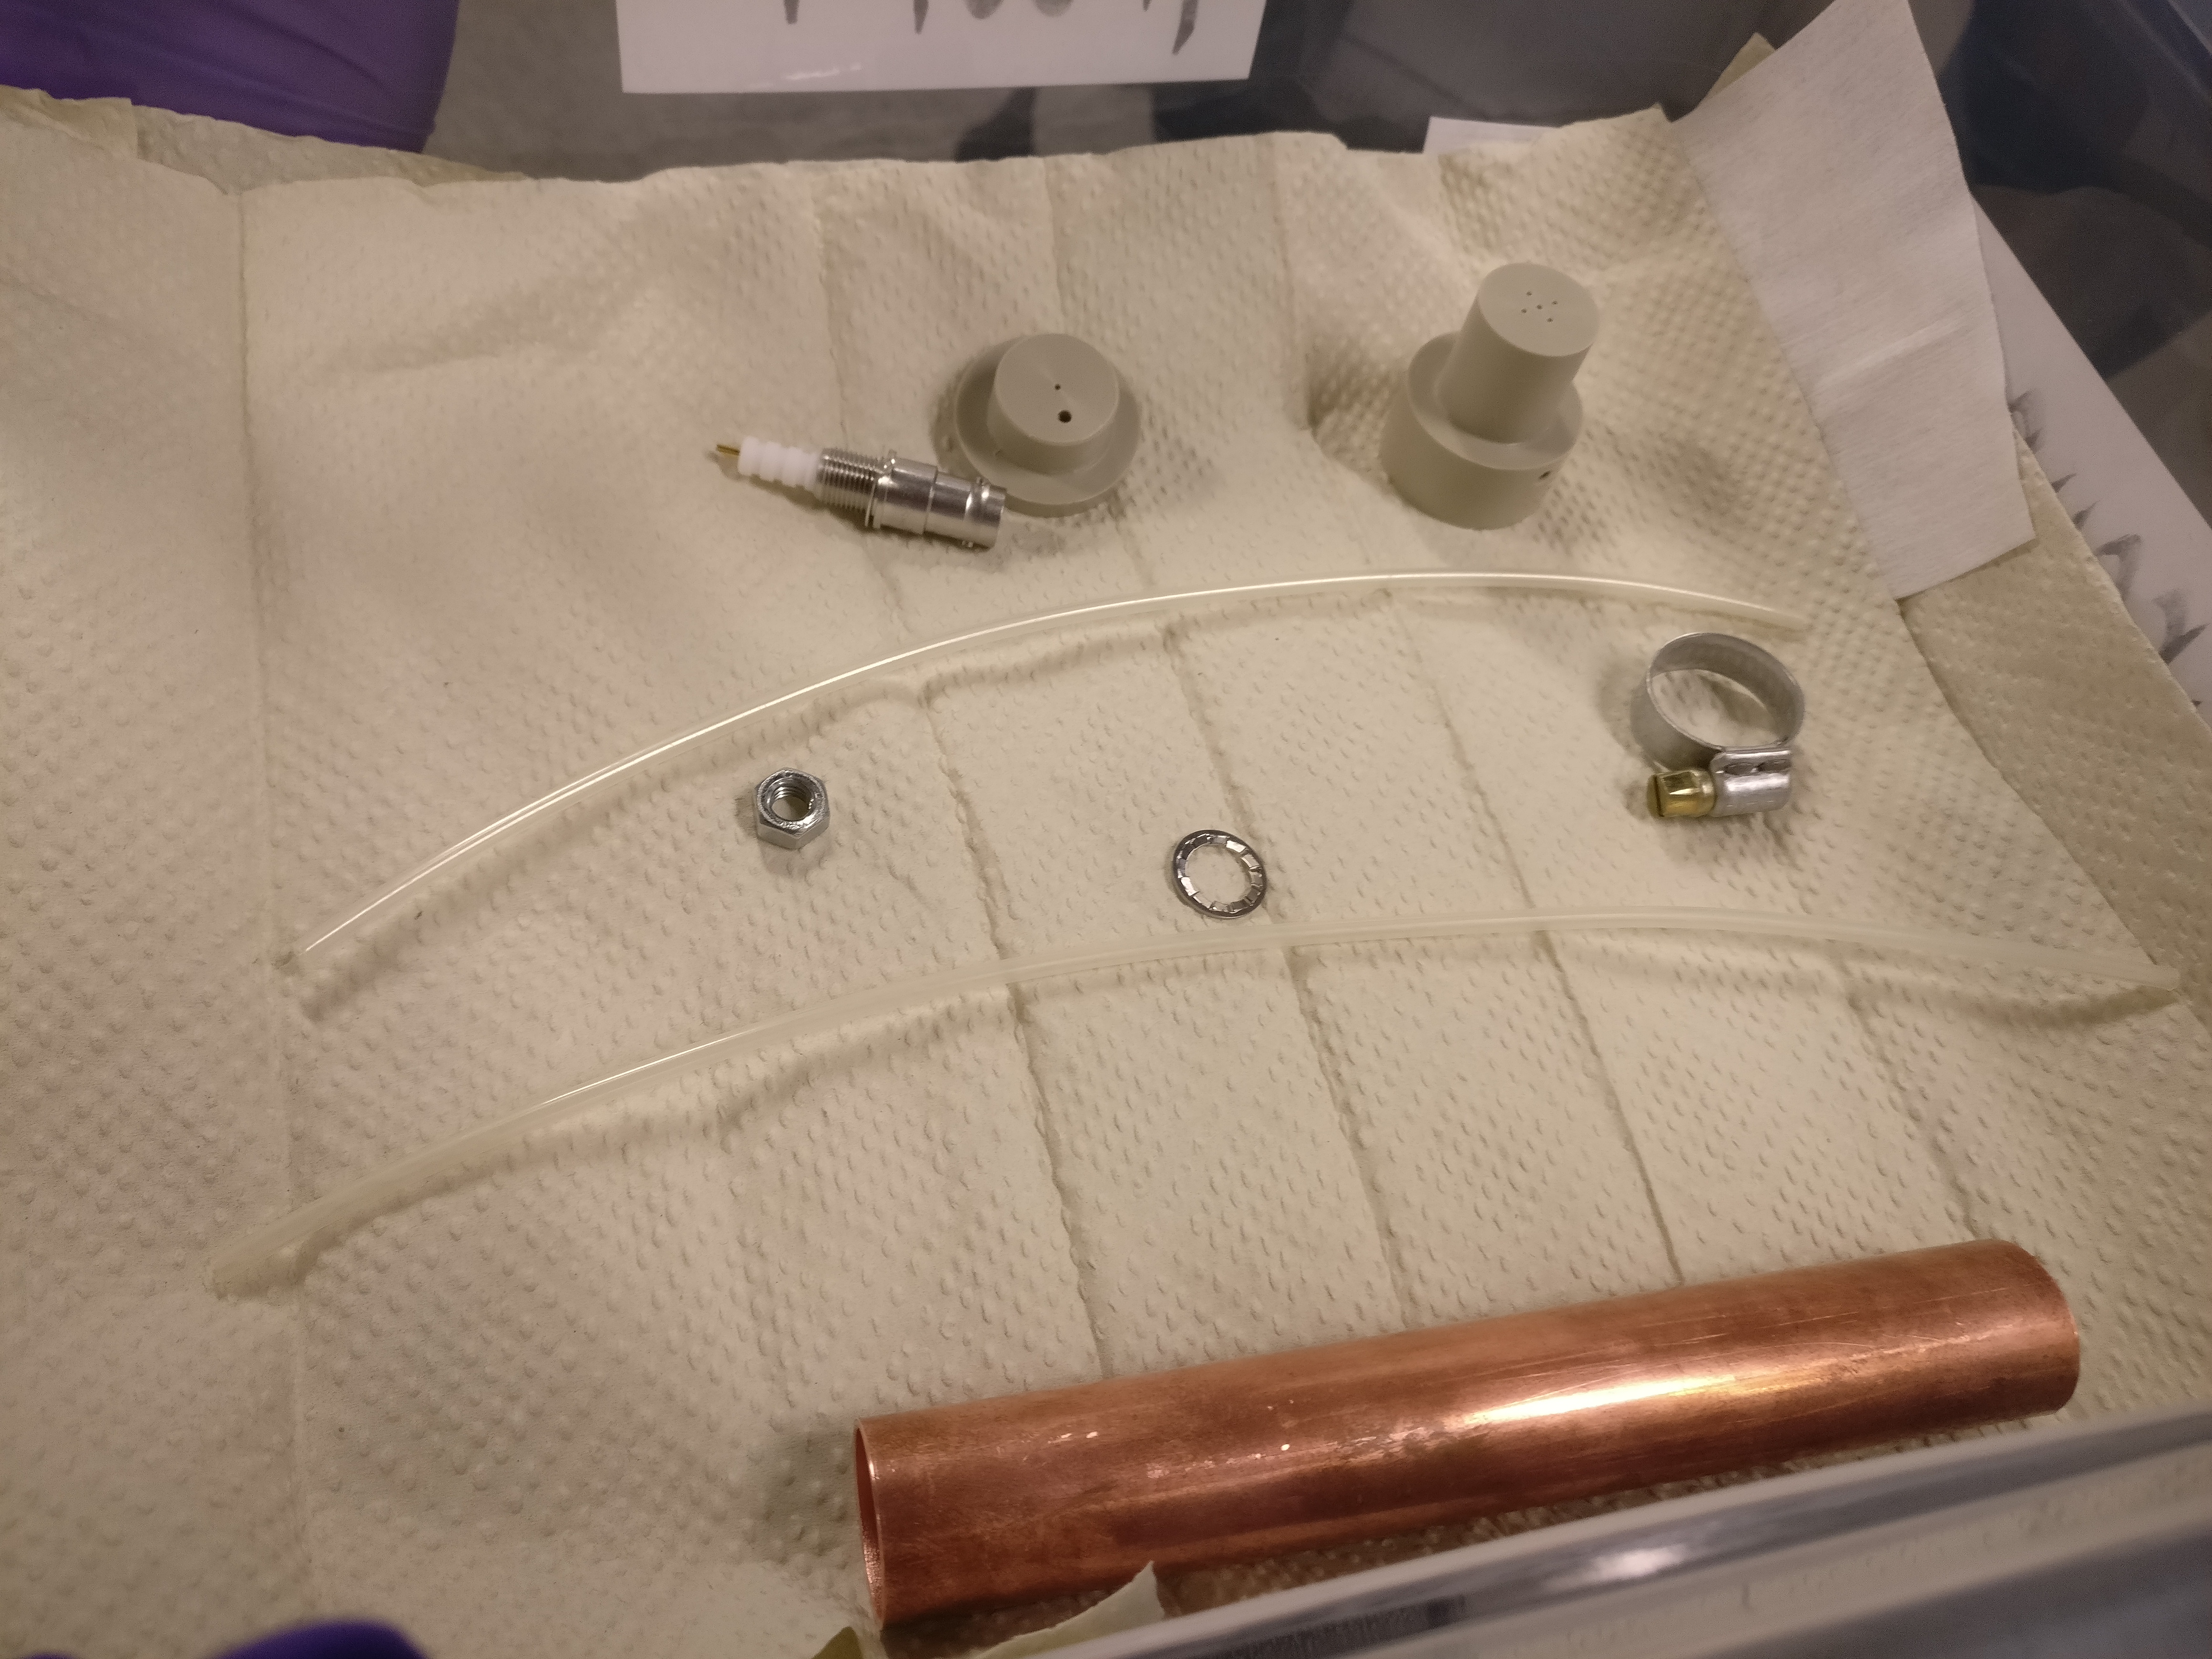
\includegraphics[width=0.5\textwidth]{./graphics/copper_tube_parts.jpg}
  \caption{Cleaned parts of the copper tube assembly}
  \label{fig:copper_parts}
\end{figure}

Finally, the hole drilled for the target was covered by a small piece of metallic tape, held in place by epoxy glue to seal off the opening.

\subsubsection{Testing}

The copper tube detector was flushed and then filled with P10 gas and connected to the amplifier electronics in a similar fashion than the previous detector. Unfortunately, preliminary observations of the signal at the oscilloscope indicated a problem with the state of the detector, as no pulses appeared on the screen even in the presence of a radioactive source. Further investigation led us to realise that the HV connector became electrically shorted when leftover parts of the anode wire (that did not get cut) came into contact with the outer part of the HV connector, as the end cap was inserted into the tube. This rendered the device inoperable, and thus we needed to rely on measurements on reference tubes to get a comparison with the can detector. Results in section \ref{sec:special_detec} have thus not been made with the instrument characterised in table \ref{Tab:coppercan_sizes}.

\begin{table}[htb!]
	\begin{tabularx}{\linewidth}{p{4.5cm}r}
		\textbf{Element} & \textbf{Mean}~{[}mm{]}          \\ \hline
		Copper tube, length            & $149.08 \pm 0.02$ \\
		Copper tube, wall thickness    & $1.04 \pm 0.04$  \\
		Copper tube, inner diameter    & $19.91 \pm 0.11$  \\
		Copper tube, radiation hole    & $5.05 \pm 0.03$  \\
		HV frontend,  total length         & $36.79 \pm 0.04$  \\
		HV frontend, top part length       & $15.90 \pm 0.04$  \\
		HV frontend, tube extremity radius & $19.85 \pm 0.01$  \\
		backend, total length             & $14.97 \pm 0.07$  \\
		backend, top part length          & $4.99 \pm 0.05$  \\
		backend, tube extremity radius    & $19.87 \pm 0.01$  \\
		Brass tube diameter            & $1.000$           \\
		Anode wire thickness           & $0.025$           \\ \hline
	\end{tabularx}
\caption{Measurements of the copper pipe experiment setup components. Measurements without uncertainties were only measured once and are dominated by the systematic uncertainties of the measurement tools. The ends are made of Teflon.}
\label{Tab:coppercan_sizes}
\end{table}




















    % Fabian
        
	\clearpage
	\section{Experimental setup Calibration}

\subsection{Set-up}
Before performing the source spectra measurements, the detector was connected to the HV power supply and to an amplifying circuit consisting of a \textit{preamplifier} and a \textit{coarse-gain amplifier}, shown on respectively in figure \ref{fig:preamp_photo} and \ref{fig:ampli_gene}. 

\begin{figure}[ht]
  \includegraphics[width=\textwidth]{graphics/preamplifier.jpg}
  \caption{Photograph of the preamplifier unit.}
  \label{fig:preamp_photo}
\end{figure}

\begin{figure}[ht]
  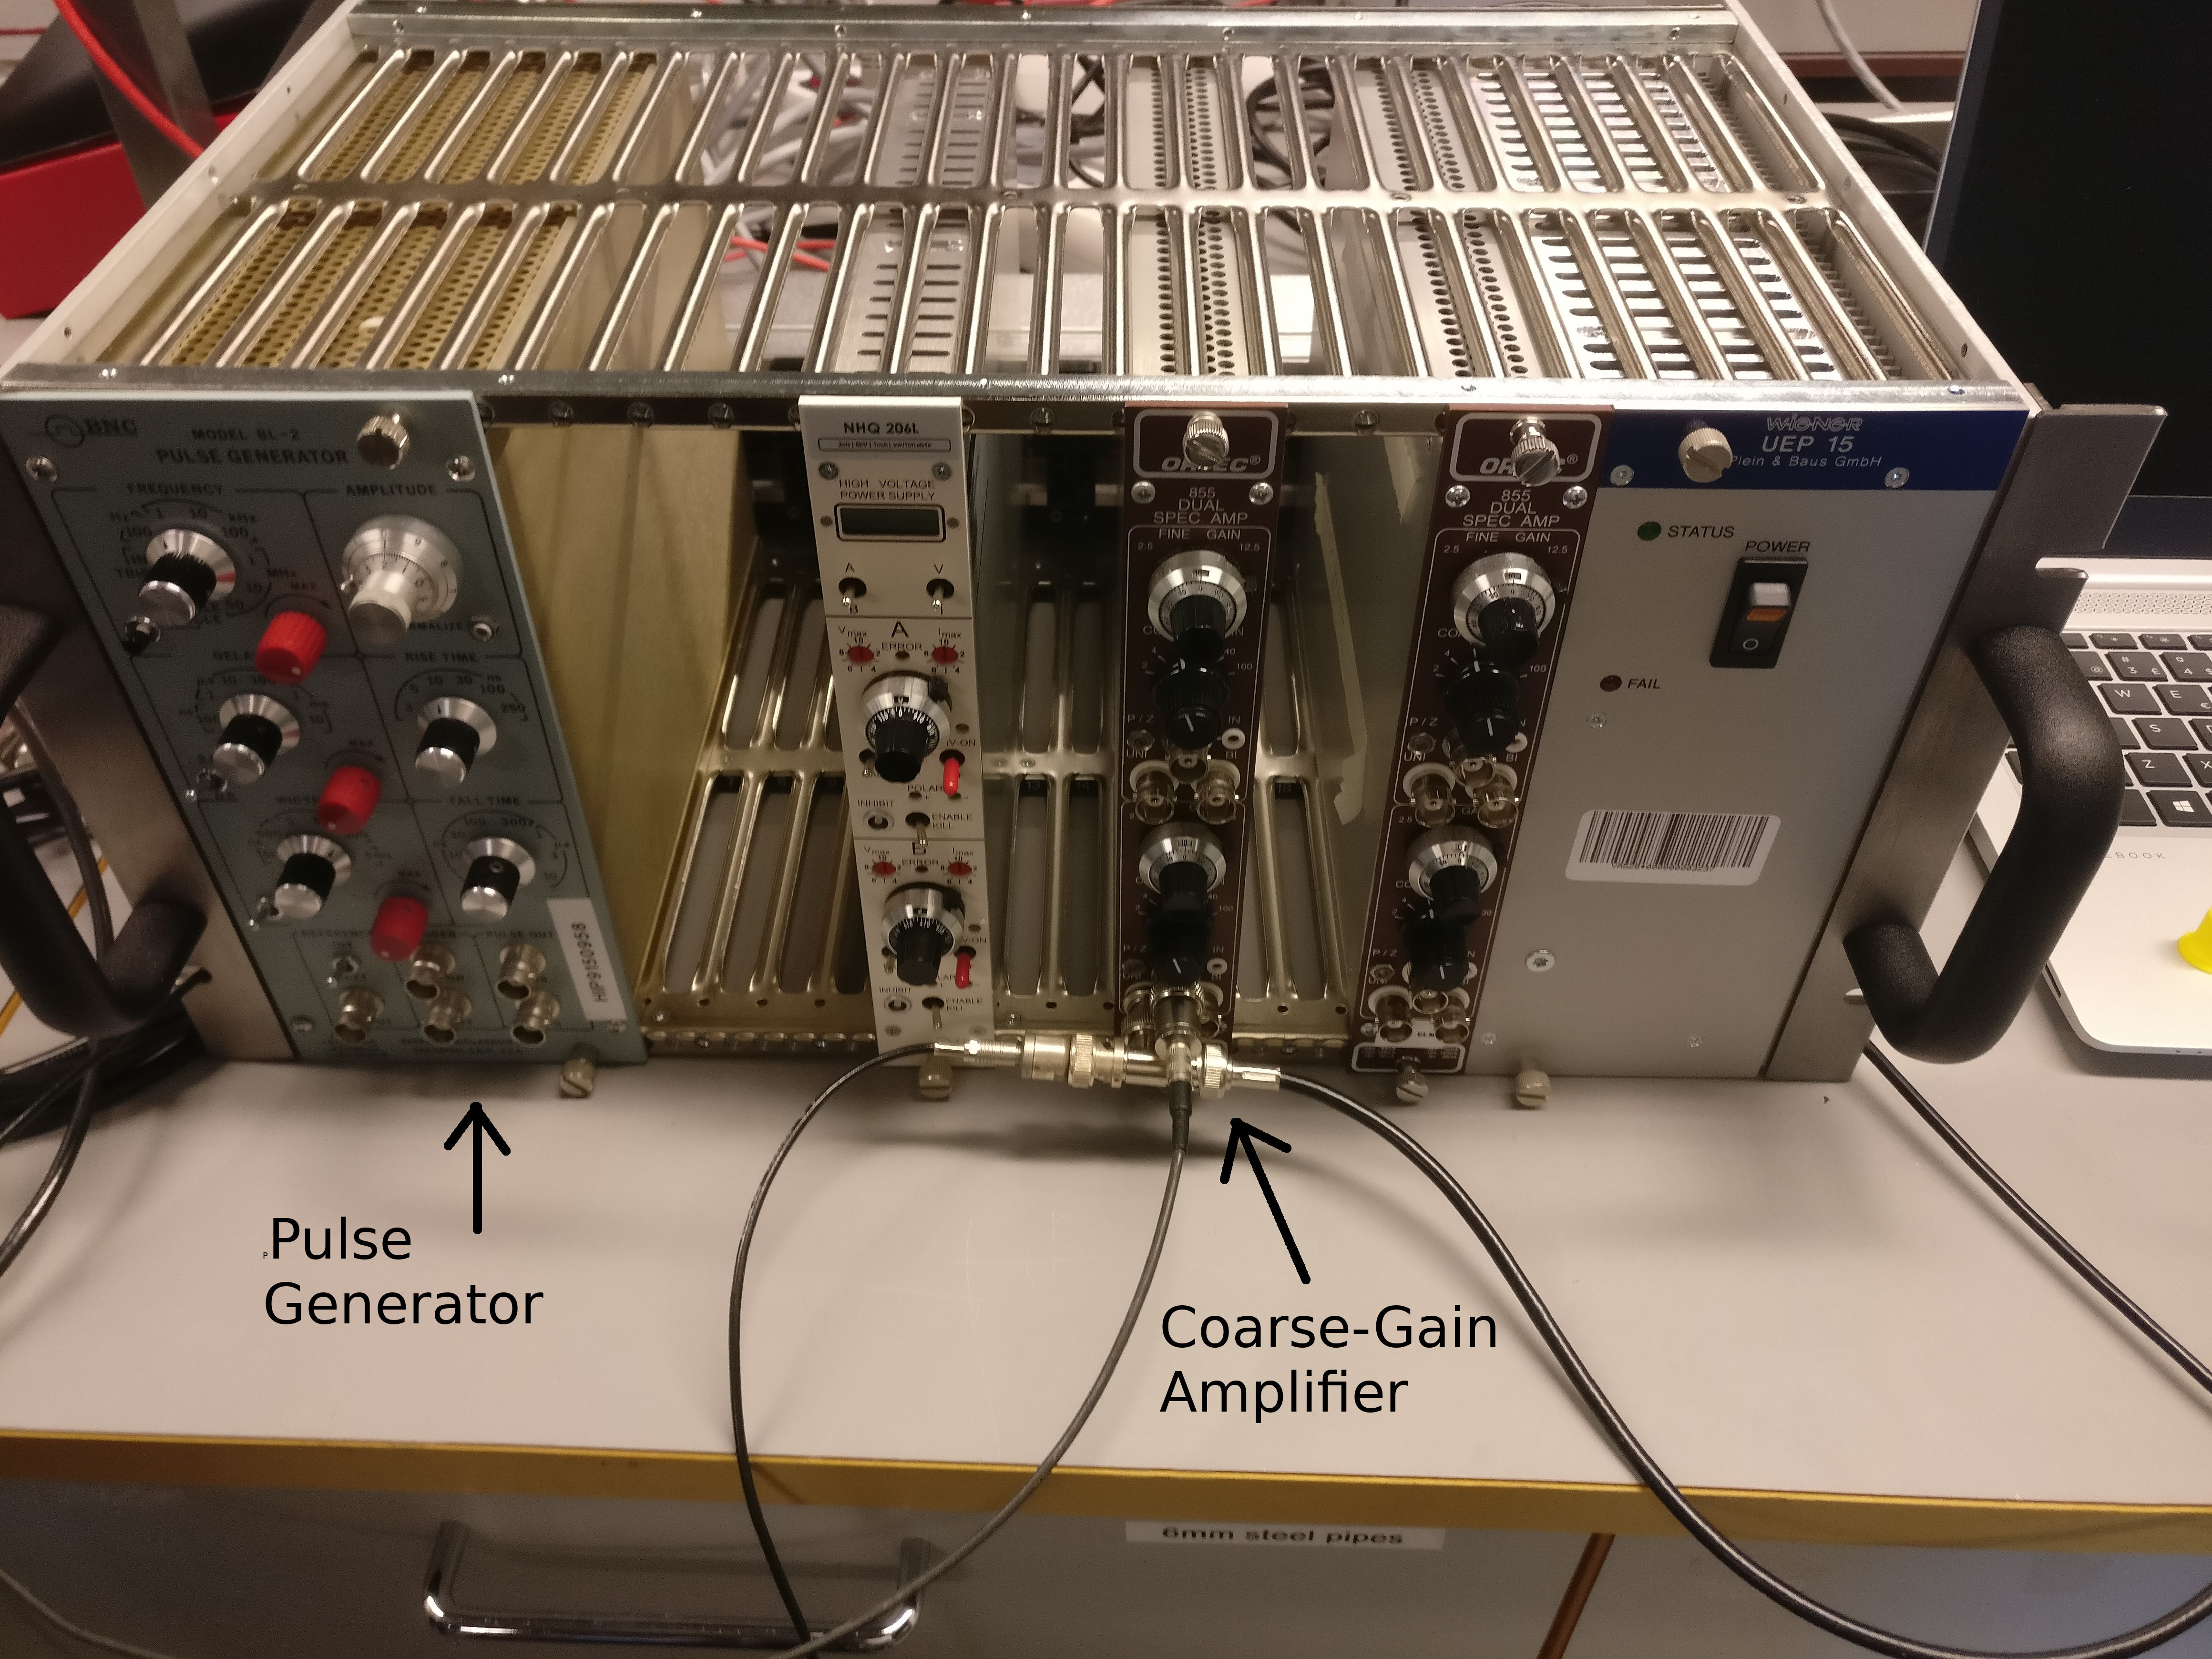
\includegraphics[width=\textwidth]{graphics/amplifier_photo.jpg}
  \caption{Photograph of the pulse generator used to inject pulses into the preamplifer, and the coarse gain amplifier used in front of the MCA}
  \label{fig:ampli_gene}
\end{figure}

Both system contribute to increase the overall number of signal electrons collected per avalanche occuring in the drift chamber. The overall gain in signal, between the drift chamber electrode and the final Multi-Channel Analyzer (MCA) reading out data, is given by equation \ref{eq:gain_system}.

\begin{equation}
  \label{eq:gain_system}
  Q_{MCA} = Q_{drift}\cdot G_{pre}\cdot G_{coarse}
\end{equation}


\subsection{Calibration of the pre-amplifier gain}
 Calibrated pulses of various intensities were injected into the electronics, and the output was displayed onto an oscilloscope to evaluate the gain of the preamplifier, $G_{pre}$ and its uncertainty.


\begin{figure}[ht]
  \includegraphics[width=\textwidth]{graphics/preamp_gain_calibration.png}
  \caption{Output voltage of pulses injected into the pre-amplifier electronics.}
  \label{fig:preamp_gain}
\end{figure}


\subsection{Calibration of the Coarse Gain amplifier}
To estimate the uncertainty on the coarse gain amplifier, subsequent runs of Fe$^{55}$ and Am$^{241}$ spectra acquisitions were made at the same operating voltage, but different coarse gain settings. Figure \ref{fig:coarse_gain} shows the result of this analysis. Since the data acquired only allowed us to measured \textit{ratios} of gain settings, the uncertainties of the absolute amplifier gain are simply assumed to scale with the lowest gain setting possible. In other words, the amplifier gain at a particular setting can be defined as:

\begin{equation}
  \label{eq:gain_abs}
  G_{coarse} = 2\cdot\Pi_{i>2}^{i=j}\frac{G_{i}}{G_{i-1}}
\end{equation}

where $j$ is the gain level at which the amplifier is operated. Figure \ref{fig:coarse_gain} presents the various ratios of gain settings measured, using both the Fe$^{55}$ and Am$^{241}$ source. The red data point show the result of combining both results, which allows us to get better estimates of the gain ratio uncertainties.

\begin{figure}[ht]
  \includegraphics[width=\textwidth]{graphics/coarse_gain_calibration.png}
  \caption{Determination of the coarse gain amplification uncertainties. Results are presented in the form of gain ratios between every adjacent setting of the coarse gain knob. The combined value and uncertainty on each measurement is shown by the red data points.}
  \label{fig:coarse_gain}
\end{figure}


    % Etienne

	\clearpage
	\section{Energy scale calibration}
\label{sec:energy_scan}

\subsection{Resolution Scans}
\label{sec:resolution_scans}
As the signal from the detector is rather weak, the detector is connected to an
amplifying circuit as described in Sec.~\ref{sec:calibration:set-up}. However
there is a trade-off associated with this procedure as amplification also
applies to noise in the detector. In order to increase the signal strength the
voltage applied to the detector can be increased which in turn increases the
amount of signal electrons and leads to a stronger output signal. Along with
this comes though an increased probability for spontaneous discharges along
impurities and dirt remaining in the detector despite extensive cleaning
procedures as described in Sec.~\ref{sec:construction}.

As the two possibilities for varying the output signal strength are associated
with independent increases of noise and accordingly reduction of resolution we
are performing resolution scans for the two samples we are interested in
measuring: Americium and Iron.

In order to reliably determine the resolution a Gaussian is fitted to the sample
peak previously identified in the MCA spectrum. We look
at the variable peak width divided by the peak position in order to determine
the resolution of our peak. For the peak width we are using the full-width
half-maximum (FWHM) value. As secondary decays will affect especially the lower
end of the decay Gaussian \todo[inline]{how are they called exactly? secondary seems
  wrong} shape we are defining regions of interest (ROI) in which the Gaussian
is fitted.

The spectra obtained for americium (Fig \ref{fig:scan:americium}) and iron
(Fig. \ref{fig:scan:iron}) are presented in appendix~\ref{app:resolution-scans} for different gains and voltages.
A Gaussian is fitted to the marked ROI (blue lines) and the obtained channel number as well as
full-width half-maximum (FWHM) in channels are denoted in each figure.

The obtained parameters from the fit are plotted in Fig.
\ref{fig:resolution:americium} and \ref{fig:resolution:iron} for americium and
iron respectively. The uncertainties are propagated from the fit. Additionally to the
total uncertainty on the FWHM, a \SI{10}{\percent} systematic
uncertainty was added due to the dependency on choosing the corresponding ROI.

\begin{figure}[htb]
  \includegraphics[width=\linewidth]{graphics/americium_scan}
  \caption{Americium scan}
  \label{fig:resolution:americium}
\end{figure}

\begin{figure}[htb]
  \includegraphics[width=\linewidth]{graphics/iron_scan}
  \caption{Iron scan}
  \label{fig:resolution:iron}
\end{figure}


%%%%%%%%%%%%%%%%%%%%%%%%%%%%%%%%%%%%%%%%%%%%
% Charge multiplication
%%%%%%%%%%%%%%%%%%%%%%%%%%%%%%%%%%%%%%%%%%%%

\section{Charge Multiplication}
\label{sec:systematics}

In Sec. \ref{sec:energy_scan} the resolution for each voltage (with its coarse gain) is calculated by finding the FWHM and the mean of the characteristic peak of the two materials.
The same data can be used to calculate the collected charge as a function of the applied voltage. In fact, the MCA mean of the peaks can be converted in an amount of charge using the calibration curve in Fig. \ref{fig:charge_calibration}. Since the data in Fig. \ref{fig:resolution:americium} and \ref{fig:resolution:iron} are taken at different coarse gains and the calibration data are collected with coarse gain $10$, a factor needs to be applied to correct for the difference, with the factor being $10/G_{coarse}$. For each measurement $i$, then, the collected charge is calculated as such:

\begin{adjustwidth}{-1cm}{}
\begin{align}
Q_{coll, i} = (b + a \cdot mean_{MCA, i}) \cdot \frac{10}{G_{coarse, i}} 
\end{align}
\end{adjustwidth}

where $Q_{coll, i}$ is the collected charge per measurement, $a$ and $b$ are the calibration function parameters from Fig. \ref{fig:charge_calibration}, $mean_{MCA, i}$ is the mean of the gaussian in the MCA spectrum and $G_{coarse, i}$ is the coarse gain used for the measurement. In order to obtain the number of electrons, $Q_{coll, i}$ is then divided by the charge of one electron $1.602 \cdot 10^{-19}$ C. The results for both Am and Fe are shown in Fig. \ref{fig:number_of_electrons}, where the errorbars are smaller than the data points. The uncertainties on these points are both statistial and systematics and they are combined in quadrature; in particular, the systematic uncertainties come from the systematic uncertainties on $mean_{MCA, i}$ and on $G_{coarse, i}$.


\begin{figure}[htb]
  \includegraphics[width=0.5\textwidth]{graphics/numbervsvoltage.pdf}
  \caption{Charge collected in the cider can proportional detector as a function of the voltage applied for the Fe and Am sources. Note that the errorbars are smaller than the plotted points.}
  \label{fig:number_of_electrons}
\end{figure}

After having calculated the number of electrons collected as a function of voltage, we can find the measured multiplication factor per measurement $i$ as

\begin{align}
\label{eq:Mexp}
M_{experimental,i} &= \frac{N_{carriers,out,i}}{N_{carriers per avalanche}} \nonumber \\
                   &= \frac{Q_{coll,i}}{n_{Fe^{5},Am^{241}}\cdot e}
\end{align}

where $M_{experimental,i}$ is the experimentally measured multiplication factor, $Q_{coll,i}$ is the charge collected per measurement, $e$ is the electron charge and $n_{Fe^{55},Am^{241}}$ is the average number of electrons-ion pairs produced by either Fe$^{55}$ (227) or Am$^{241}$ (2290), as taken from \cite{can_paper}.

In order to compare those found values with the theoretical expectation, we computed the multiplication factor with the parameters of our experiment (and of the environment the experiment was conducted in) using this formula, which assumes that our detector is operating in the linear regime (\cite{gas_detect}):

\begin{adjustwidth}{+0.5cm}{}
\begin{align}
\ln(M)=\frac{\ln(2)}{\ln(r_{c}/r_{a})}\cdot\frac{V}{\Delta V}\cdot\ln\left[ \frac{V\rho_{o}}{ra\ln(r_{c}/r_{a})E_{min}(\rho_{o})\rho}\right]
\label{eq:lnm}
\end{align}
\end{adjustwidth}

The meaning and values associated with each parameter of this equation is listed in Tab. \ref{Tab:params}. One can see that most of these values either come from tabulated properties of the gas used, or are derived from the initial measurement of the beer can dimensions, listed in Tab. \ref{Tab:cidercan_sizes} for reference.

\begin{table*}[htb]
  \begin{tabularx}{\linewidth}{p{1.5cm}p{8cm}rl}
    \textbf{Variable}     & \textbf{Definition}                                                         & \textbf{Value}     & \textbf{Source}  \\
    \hline
    $r_{c}$                 & radius of the cathode                                                       & $3.121 \pm 0.003$      & Eq. \ref{eq:rcra}   \\
    &&&\\
    $r_{a}$                 & radius of the anode                                                         & $\SI{25 +- 2}{\micro\meter}$ & Eq. \ref{eq:rcra}   \\
    &&&\\
    $V$                    & operating voltage                                                           & 1-3 kV             & N/A                \\
    &&&\\
    $\Delta V$             & potential required to produce an additional electron                & $23.6 \pm 5.4$ V   &\cite{gas_detect}   \\
    &&&\\
    $E_{min}(\rho_{o})$      & \begin{tabular}[c]{@{}l@{}}Minimal electric field needed for ionisation\\(at standard pressure)\end{tabular}         & $48. \pm 3$ kV/cm  &\cite{gas_detect}   \\
    &&&\\
    $\rho_{o}/\rho$ & \begin{tabular}[c]{@{}l@{}}Standard density of the gas\\(compared to density at  T=273K and P = 1 bar)\end{tabular}  &                    &Eq. \ref{eq:gaslaw}, \cite{meteo}\\
    \hline
  \end{tabularx}
  \caption{List of the main systematics sources}
  \label{Tab:params}
\end{table*}

For the geometric properties, the relationship between the measured quantities and the anode radius, is simply $r_{a} = d_{a}/2$, with $d_{a}$ being the radius of the anode wire. Meanwhile, the radii of the cathode is related to the other measurements via Eq. \ref{eq:rcra}.

\begin{align}
  \label{eq:rcra}
  r_{c} = \frac{D_{outer}}{2}-\tau
\end{align}

where $D_{outer}$ is the outer radius of the cider can and $\tau$ is the can wall thickness.
To determine the gas properties at the environmental conditions of the laboratory, the temperature and pressure of the room need to be measured. With these values on hand, the ratio of gas densities can be determined by using the ideal gas law.

\begin{align}
  \label{eq:gaslaw}
  \frac{\rho}{\rho_{o}} = \frac{P}{P_{o}}\cdot \frac{T_{o}}{T}
\end{align}

with $\rho$ being the gas density, $P$ the gas pressure and $T$ its temperature.
During the measurements, the temperature stayed mostly constant, but the pressure varied over the course of the day, as shown in Fig. \ref{fig:pressure}. The uncertainty on the pressure was thus selected to be the largest pressure change with respect to standard pressure, over the course of a day.

\begin{figure}[htb]
  \includegraphics[width=0.5\textwidth]{graphics/pressure_monitoring.png}
  \caption{Atmospheric pressure in Helsinki during the spectra measurement. Source: \cite{meteo}}
  \label{fig:pressure}
\end{figure}

Given the parameters and uncertainties quoted in Tab. \ref{Tab:params}, a MC simulation was created in order to compute the theoretical uncertainties on the expected multiplication factor as a function of operating voltage. In this systematics treatment, each parameter was drawn out of Gaussian shaped probability distribution, with a mean centred at a parameter's value and the width set as the quoted uncertainty. Fig. \ref{final_lnm} shows the 1$\sigma$ and 2$\sigma$ confidence interval of the multiplication factor, after propagation of systematic uncertainties.


%The theoretical expectation for the drift chamber's electron yield can be compared to the data obtained during the iron spectrum scan described in Sec. \ref{sec:resolution_scans}. Given a number of MCA counts $Q_{mca}$, the charge accumulated at the electrodes of the drift chamber can be obtained with Eq. \ref{eq:M_exp}.

%\begin{align}
%  \label{eq:M_exp}
%  Q_{detector} = \frac{Q_{MCA}}{G_{pre,mca}\cdot{G_{coarse}}}
%\end{align}

%where $G_{pre,mca}$ is the preamplifier gain in units of $d.c./V$ (as plotted in Fig. \ref{fig:preamp_gain_mca}),and $G_{coarse}$ is the coarse gain that was described and measured in Sec. \ref{sec:coarse}. From that point, the multiplication factor of the experimental data is given by Eq. \ref{eq:Mexp}.

%\begin{align}
%  \label{eq:Mexp}
%  M_{experimental} &= \frac{N_{carriers,out}}{N_{carriers per avalanche}} \nonumber \\
%                   &= \frac{Q_{detector}}{n_{Fe^{5},Am^{241}}\cdot e}
%\end{align}

%Where $n_{Fe^{55},Am^{241}}$ is the average number of electrons-ion pairs produced by either Fe$^{55}$ (227) or Am$^{241}$ (2290), as taken from \cite{can_paper}. 

The measured multiplication factors obtained in each voltage scan is shown in Fig. \ref{final_lnm}, along with the theoretical expectation for their values given the geometry of the can detector and the environmental conditions during the measurement. As one can see, the data collected lies within the $1\sigma$ band of the theoretically predicted values.

\begin{figure}[htb]
  \includegraphics[width=0.5\textwidth]{graphics/lnM_final_plot.pdf}
  \caption{Natural logarithm of the drift chamber's multiplication factor M. Red and green data points represent the results obtained with $Fe^{55}$ and $Am^{241}$ respectively. Blue bands show the theoretical expectation for the detector, given systematics uncertainties in the cider can geometry and gas properties.}
  \label{final_lnm}
\end{figure}
 % Daniel

        \clearpage
	\section{Spectra analysis}

\subsection{Fe$^{55}$}

\subsection{Am$^{81}$}
         % Daniel

        \clearpage
	\section{Analysis of systematics}
\label{sec:systematics}
In the analysis of data from experiments, care must be taken to properly take into account systematic uncertainties in our measurements. In the case of the cider can detector, environmental and geometric factors can influence the overall performances of the drift chamber, namely the average number of carriers produced and collected at the electrodes. This number, called the \textit{gain} or \textit{multiplication factor}, can be approximated by the following formula, assuming that our detector is operating in the linear regime(\cite{gas_detect}):

\begin{equation}
  \label{eq:lnm}
  \ln(M)=\frac{\ln(2)}{\ln(r_{c}/r_{a})}\cdot\frac{V}{\Delta V}\cdot\ln\left[ \frac{V\rho_{o}}{ra\ln(r_{c}/r_{a})E_{min}(\rho_{o})\rho}\right]
\end{equation}

The meaning and values associated with each parameter of this equation is listed in table \ref{Tab:params}. One can see that most of these values either come from tabulated properties of the gas used, or are derived from the initial measurement of the beer can dimensions, listed in table \ref{Tab:cidercan_sizes} for reference.

\begin{table}[htb]
  \begin{tabularx}{\linewidth}{p{1.5cm}|p{6cm}|c|l}
    \textbf{Variable}     & \textbf{Definition}                                                         & \textbf{Value}     & \textbf{Source}  \\
    \hline
    $r_{c}$                 & radius of the cathode                                                       & $3.121 \pm 0.003$      &\ref{eq:rcra}   \\
    &&&\\
    $r_{a}$                 & radius of the anode                                                         & $25 \pm 2 \mu$m &\ref{eq:rcra}   \\
    &&&\\
    $V$                    & operating voltage                                                           & 1-3 kV             & N/A                \\
    &&&\\
    $\Delta V$             & average potential required to produce an additional electron                & $23.6 \pm 5.4$ V   &\cite{gas_detect}   \\
    &&&\\
    $E_{min}(\rho_{o})$      & Minimal electric field needed for ionization (at standard pressure)         & $48. \pm 3$ kV/cm  &\cite{gas_detect}   \\
    &&&\\
    $\frac{\rho_{o}}{\rho}$ & Standard density of the gas (compared to density at  T=273K and P = 1 bar)  &                    &\ref{eq:gaslaw}, \cite{meteo}\\
    \hline
  \end{tabularx}
  \caption{List of the main systematics sources}
  \label{Tab:params}
\end{table}


\begin{table}[htb]
  \begin{tabularx}{\linewidth}{X|X|p{2cm}}
    \textbf{Element}                   & \textbf{Measurements}                                 & \textbf{Size}       \\ \hline
    Cider can diameter $D_{outer}$      &                                                       &                     \\
    Cider can wall thickness   $\tau$ & $105 \pm 10 \ \mu$m                                   & $105 \pm 10 \ \mu$m \\
    Plastic tube diameter             & $5.89$ mm, $5.95$ mm, $6.00$ mm, $6.01$ mm, $6.01$ mm &                     \\
    Brass tube diameter               & $1.0$ mm                                              &                     \\
    Nylon screw diameter              & $7.8$ mm, $7.75$ mm                                   &                     \\
    HV connector diameter             & $9.37$ mm                                             &                     \\
    Anode wire diameter               & $50 \pm 10 \ \mu$m                                    & $50 \pm 10 \ \mu$m  \\
    \hline
  \end{tabularx}
  \caption{Measurements of the cider can experiment setup components.}
  \label{Tab:cidercan_sizes}
\end{table}

For the geometric properties, the relationship between the measured quantities and the anode radius, is simply $r_{a} = d_{a}/2.$. Meanwhile, the radii of the cathode is related to the other measurements via equation \ref{eq:rcra}.

\begin{equation}
  \label{eq:rcra}
  r_{c} = \frac{D_{outer}}{2}-\tau
\end{equation}

To determine the gas properties at the environmental conditions of the laboratory, one needed to measure the temperature and pressure of the room. With these values on hand, the ratio of gas densities can be determined by using the ideal gas law.

\begin{equation}
  \label{eq:gaslaw}
  \frac{\rho}{\rho_{o}} = \frac{P}{P_{o}}\cdot \frac{T_{o}}{T}
\end{equation}

During the measurements, the temperature stayed mostly constant, but the pressure varied over the course of the day, as shown in figure \ref{fig:pressure}. The uncertainty on the pressure was thus selected to be the largest pressure change with respect to standard pressure, over the course of a day.

\begin{figure}[htb]
  \includegraphics[width=\textwidth]{graphics/pressure_monitoring.png}
  \caption{Atmospheric pressure in Helsinki during the spectra measurement. Source: \cite{meteo}}
  \label{fig:pressure}
\end{figure}

Given the parameters and uncertainties quoted in table \ref{Tab:params}, a MC simulation was created in order to compute the theoretical uncertainties on the expected multiplication factor as a function of operating voltage. In this systematics treatment, each parameter was drawn out of gaussian shaped probability distribution, with a mean centered at a parameter's value and the width set as the quoted uncertainty. Figure \ref{fig:final_lnm} shows the 1$\sigma$ and 2$\sigma$ confidence interval of the multiplication factor, after propagation of systematic uncertainties.

The theoretical expectation for the drift chamber's electron yield can be compared to the data obtained during the iron spectrum scan described in section \ref{sec:voltage_calibration}. Given a number of MCA counts $Q_{mca}$, the charge accumulated at the electrodes of the drift chamber can be obtained with equation \ref{eq:M_exp}.

\begin{equation}
  \label{eq:M_exp}
  Q_{detector} = \frac{Q_{MCA}}{G_{pre,mca}\cdot{G_{coarse}}}
\end{equation}

where $G_{pre,mca}$ is the preamplifier gain in units of $d.c./V$ (as plotted in figure \ref{fig:preamp_gain_mca}),and $G_{coarse}$ is the coarse gain that was described and measured in section \ref{sec:coarse}. From that point, the multiplication factor of the experimental data is given by the following:

\begin{equation}
  M_{experimental} = \frac{N_{carriers,out}}{N_{carriers per avalanche}} = \frac{Q_{detector}}{n_{Fe^{5},Am^{241}}\cdot e}
\end{equation}

Where $n_{Fe^{5},Am^{241}}$ is the average number of electrons-ion pairs produced by either iron-55 (227) or americium-241 (2290), as taken from \cite{can_paper}. The measured multiplication factors obtained in each voltage scan is shown in figure \ref{final_lnm}, along with the theoretical expectation for their values given the geometry of the can detector and the environmental conditions during the measurement. As one can see, the data collected is matches remarkably well the prediction, which has its $1\sigma$ and $2\sigma$ contours plotted in blue.

\begin{figure}[H]
  \includegraphics[width=\textwidth]{graphics/lnM_final_plot.png}
  \caption{Natural logarithm of the drift chamber's multiplication factor M. Red and green data points represent the results obtained with $Fe^{5}$ and $Am^{241}$ respectively. Blue bands show the theoretical expectation for the detector, given systematics uncertainties in the cider can geometry and gas peroperties.}
  \label{final_lnm}
\end{figure}

     % Etienne
        
	\clearpage
	\section{Special Detector results}
\label{sec:special_detec}


 % 
	
	\clearpage
	\section{Conclusion}
The laboratory work conducted here can be concluded by a succesful build and
operation of a proportional gas detector based on a cider can. A different setup
with a copper tube has also been constructed but was not operational due to a
electrical short between the andode wire and the outer part of the HV connector.
Supplied data was instead analysed in this report for copper and aluminium
tubes.

The amplifying circuit used to measure the voltage from the detector has been
succesfully calibrated and found a gain of the preamplifier of
$G_\mathrm{pre}=\SI{6.413 \pm 0.005}{}$ and the uncertainty on the coarse gain was
determined to be ${\sigma_{G_\mathrm{coarse}} = 0.3}$.

Herafter a resolution scan has been performed varying both voltage and amplifier
gain to determine the optimal setting for the two samples of interest: Fe$^{55}$
and Am$^{241}$. Using a \SI{10}{\percent} uncertainty for the selection of
region of interest for performing fits yielded good results at \SI{1937}{\volt}
and a gain of $4$ for both samples. Additionally the charge collected by the
cider can detector has been compared to theoretical expecation under the
assumption that the detector is operating in the linear regime, and
an agreement within $1\sigma$ was found when taking into account uncertainties in
determining the detector dimensions, atmospheric pressure and voltage fluctuations.

Data collected for the two samples at optimal resolution as well as background samples have
been analysed for all detectors. Here the calibration was applied, background
subtracted using a bspline parametrization of the data and escape peaks were fitted using
Gaussians. Peaks in the spectra were succesfully identified, noted and compared
to their known values showing a near perfect match for the cider can and a good
agreement for the aluminium detector.

The \SI{10}{\percent} systematic uncertainty on the resolutions carry on into the systematic
uncertainty of the final energy measurements. The systematic uncertainties is much larger than
the statistical and calibration uncertainties, and the accuracy of the energy measurements suggests
that the systematic uncertainty is overestimated.               % Rosanna
	
	
	
	% === Appendices ======================================================	
	
  \FloatBarrier
	\cleardoublepage
	\appendix
	\onecolumn
\section{Resolution scans for Am and Fe}
\label{app:resolution-scans}
\begin{figure}[htb]
  \centering
  \foreach \n [count=\i] in {%
    am_100_1136,
    am_100_1191,
    am_100_1244,
    am_100_1297,
    am_100_1351,
    am_100_1399,
    am_40_1397,
    am_40_1455}{
   \begin{subfigure}{.42\linewidth}
        
         \includegraphics[width=\linewidth]{graphics/\n}
        \caption{\detokenize\expandafter{\n}}
      \end{subfigure}
    }
  \end{figure}
  \begin{figure}[htb]\ContinuedFloat
  \centering
  \foreach \n [count=\i] in {%
    am_40_1502,
    am_40_1559,
    am_20_1559,
    am_20_1603,
    am_20_1666,
    am_10_1665,
    am_10_1712,
    am_10_1758}{
   \begin{subfigure}{.42\linewidth}
        
         \includegraphics[width=\linewidth]{graphics/\n}
        \caption{\detokenize\expandafter{\n}}
      \end{subfigure}
    }
\end{figure}
  \begin{figure}[htb]\ContinuedFloat
  \centering
  \foreach \n [count=\i] in {%
    am_4_1757,
    am_4_1808,
    am_4_1858,
    am_4_1899,
    am_2_1900,
    am_2_1951,
    am_2_2001} {
   \begin{subfigure}{.42\linewidth}
        
         \includegraphics[width=\linewidth]{graphics/\n}
        \caption{\detokenize\expandafter{\n}}
      \end{subfigure}
    }
    \caption{Scan for different gains and voltages for Americium.}
    \label{fig:scan:americium}
\end{figure}

\begin{figure}[htb]
  \centering
  \foreach \n [count=\i] in {%
fe_100_1420,
fe_100_1470,
fe_100_1523,
fe_100_1572,
fe_100_1617,
fe_100_1717,
fe_40_1717,
fe_40_1801}{
   \begin{subfigure}{.42\linewidth}
        
         \includegraphics[width=\linewidth]{graphics/\n}
        \caption{\detokenize\expandafter{\n}}
      \end{subfigure}
    }
  \end{figure}
  \begin{figure}[htb]\ContinuedFloat
  \centering
  \foreach \n [count=\i] in {%
fe_40_1853,
fe_40_1901,
fe_20_1901,
fe_20_1978,
fe_10_1978,
fe_10_2000,
fe_10_2042,
fe_10_2080}{
   \begin{subfigure}{.42\linewidth}
        
         \includegraphics[width=\linewidth]{graphics/\n}
        \caption{\detokenize\expandafter{\n}}
      \end{subfigure}
    }
\end{figure}
  \begin{figure}[htb]\ContinuedFloat
  \centering
  \foreach \n [count=\i] in {%
fe_4_2124,
fe_4_2201,
fe_2_2201,
fe_2_2254,
fe_2_2303}{
   \begin{subfigure}{.42\linewidth}
        
         \includegraphics[width=\linewidth]{graphics/\n}
        \caption{\detokenize\expandafter{\n}}
      \end{subfigure}
    }
    \caption{Scan for different gains and voltages for Iron.}
    \label{fig:scan:iron}
  \end{figure}

\FloatBarrier



	
	% === Back matter =====================================================
	
	% References
	%\bibliographystyle{plain}
	%\bibliographystyle{acm}
	\bibliographystyle{unsrt}
	\bibliography{./sections/references}
	\clearpage
	\pagestyle{empty}
	\cleardoublepage
\end{document}
